% Options for packages loaded elsewhere
\PassOptionsToPackage{unicode}{hyperref}
\PassOptionsToPackage{hyphens}{url}
\PassOptionsToPackage{dvipsnames,svgnames,x11names}{xcolor}
%
\documentclass[
  letterpaper,
]{tufte-book}

\usepackage{amsmath,amssymb}
\usepackage{lmodern}
\usepackage{iftex}
\ifPDFTeX
  \usepackage[T1]{fontenc}
  \usepackage[utf8]{inputenc}
  \usepackage{textcomp} % provide euro and other symbols
\else % if luatex or xetex
  \usepackage{unicode-math}
  \defaultfontfeatures{Scale=MatchLowercase}
  \defaultfontfeatures[\rmfamily]{Ligatures=TeX,Scale=1}
\fi
% Use upquote if available, for straight quotes in verbatim environments
\IfFileExists{upquote.sty}{\usepackage{upquote}}{}
\IfFileExists{microtype.sty}{% use microtype if available
  \usepackage[]{microtype}
  \UseMicrotypeSet[protrusion]{basicmath} % disable protrusion for tt fonts
}{}
\usepackage{xcolor}
\setlength{\emergencystretch}{3em} % prevent overfull lines
\setcounter{secnumdepth}{-\maxdimen} % remove section numbering
% Make \paragraph and \subparagraph free-standing
\ifx\paragraph\undefined\else
  \let\oldparagraph\paragraph
  \renewcommand{\paragraph}[1]{\oldparagraph{#1}\mbox{}}
\fi
\ifx\subparagraph\undefined\else
  \let\oldsubparagraph\subparagraph
  \renewcommand{\subparagraph}[1]{\oldsubparagraph{#1}\mbox{}}
\fi


\providecommand{\tightlist}{%
  \setlength{\itemsep}{0pt}\setlength{\parskip}{0pt}}\usepackage{longtable,booktabs,array}
\usepackage{calc} % for calculating minipage widths
% Correct order of tables after \paragraph or \subparagraph
\usepackage{etoolbox}
\makeatletter
\patchcmd\longtable{\par}{\if@noskipsec\mbox{}\fi\par}{}{}
\makeatother
% Allow footnotes in longtable head/foot
\IfFileExists{footnotehyper.sty}{\usepackage{footnotehyper}}{\usepackage{footnote}}
\makesavenoteenv{longtable}
\usepackage{graphicx}
\makeatletter
\def\maxwidth{\ifdim\Gin@nat@width>\linewidth\linewidth\else\Gin@nat@width\fi}
\def\maxheight{\ifdim\Gin@nat@height>\textheight\textheight\else\Gin@nat@height\fi}
\makeatother
% Scale images if necessary, so that they will not overflow the page
% margins by default, and it is still possible to overwrite the defaults
% using explicit options in \includegraphics[width, height, ...]{}
\setkeys{Gin}{width=\maxwidth,height=\maxheight,keepaspectratio}
% Set default figure placement to htbp
\makeatletter
\def\fps@figure{htbp}
\makeatother
\newlength{\cslhangindent}
\setlength{\cslhangindent}{1.5em}
\newlength{\csllabelwidth}
\setlength{\csllabelwidth}{3em}
\newlength{\cslentryspacingunit} % times entry-spacing
\setlength{\cslentryspacingunit}{\parskip}
\newenvironment{CSLReferences}[2] % #1 hanging-ident, #2 entry spacing
 {% don't indent paragraphs
  \setlength{\parindent}{0pt}
  % turn on hanging indent if param 1 is 1
  \ifodd #1
  \let\oldpar\par
  \def\par{\hangindent=\cslhangindent\oldpar}
  \fi
  % set entry spacing
  \setlength{\parskip}{#2\cslentryspacingunit}
 }%
 {}
\usepackage{calc}
\newcommand{\CSLBlock}[1]{#1\hfill\break}
\newcommand{\CSLLeftMargin}[1]{\parbox[t]{\csllabelwidth}{#1}}
\newcommand{\CSLRightInline}[1]{\parbox[t]{\linewidth - \csllabelwidth}{#1}\break}
\newcommand{\CSLIndent}[1]{\hspace{\cslhangindent}#1}

%%%%%%%
%  FIX Makeuppercase error
%  See https://tex.stackexchange.com/q/202142/157312
\usepackage{ifxetex}
\ifxetex
\renewcommand{\textls}[2][5]{%
  \begingroup\addfontfeatures{LetterSpace=#1}#2\endgroup
}
\renewcommand{\allcapsspacing}[1]{\textls[15]{#1}}
\renewcommand{\smallcapsspacing}[1]{\textls[10]{#1}}
\renewcommand{\allcaps}[1]{\textls[15]{\MakeTextUppercase{#1}}}
\renewcommand{\smallcaps}[1]{\smallcapsspacing{\scshape\MakeTextLowercase{#1}}}
\renewcommand{\textsc}[1]{\smallcapsspacing{\textsmallcaps{#1}}}
\usepackage{fontspec}
\setmainfont{TeX Gyre Pagella}
\setsansfont{TeX Gyre Heros}[Scale=MatchUppercase]
\fi
%%%%%%%


\usepackage{pdfpages}  % for cover page
\graphicspath{{Images/}} % Make Images/ default figure path


\setlength{\parindent}{0pt}%
\setlength{\RaggedRightParindent}{0pt}
\setlength{\JustifyingParindent}{0pt}%
\setlength{\parskip}{\baselineskip}


%%
% Produces a full title page

\renewcommand{\maketitlepage}[0]{%
  \cleardoublepage%
  {%
  \sffamily%
  \begin{fullwidth}%
  \fontsize{12}{14}\selectfont\par\noindent\textcolor{darkgray}{\allcaps{\thanklessauthor}}%
  \vspace{12.5pc}%
  \fontsize{20}{28}\selectfont\par\noindent\textcolor{darkgray}{\allcaps{\thanklesstitle}}%
  \vfill%
  \fontsize{10}{12}\selectfont\par\noindent\allcaps{\thanklesspublisher}%
  \end{fullwidth}%
  }
  \thispagestyle{empty}%
  \clearpage%
}

% \usepackage{beramono}
% \usepackage{ifpdf}
% \usepackage{mathpazo}
% \usepackage{letterspace}
% \usepackage{soul}

% DEFINITIONS


% The fancyvrb package lets us customize the formatting of verbatim
% environments.  We use a slightly smaller font.
\usepackage{fancyvrb}
\fvset{fontsize=\normalsize}

%%
% Prints argument within hanging parentheses (i.e., parentheses that take
% up no horizontal space).  Useful in tabular environments.
\newcommand{\hangp}[1]{\makebox[0pt][r]{(}#1\makebox[0pt][l]{)}}

%%
% Prints an asterisk that takes up no horizontal space.
% Useful in tabular environments.
\newcommand{\hangstar}{\makebox[0pt][l]{*}}

%%
% Prints a trailing space in a smart way.
\usepackage{xspace}

%%
% Some shortcuts for Tufte's book titles.  The lowercase commands will
% produce the initials of the book title in italics.  The all-caps commands
% will print out the full title of the book in italics.
\newcommand{\vdqi}{\textit{VDQI}\xspace}
\newcommand{\ei}{\textit{EI}\xspace}
\newcommand{\ve}{\textit{VE}\xspace}
\newcommand{\be}{\textit{BE}\xspace}
\newcommand{\VDQI}{\textit{The Visual Display of Quantitative Information}\xspace}
\newcommand{\EI}{\textit{Envisioning Information}\xspace}
\newcommand{\VE}{\textit{Visual Explanations}\xspace}
\newcommand{\BE}{\textit{Beautiful Evidence}\xspace}

\newcommand{\TL}{Tufte-\LaTeX\xspace}

% Prints the month name (e.g., January) and the year (e.g., 2008)
\newcommand{\monthyear}{%
  \ifcase\month\or January\or February\or March\or April\or May\or June\or
  July\or August\or September\or October\or November\or
  December\fi\space\number\year
}


% Prints an epigraph and speaker in sans serif, all-caps type.
\newcommand{\openepigraph}[2]{%
  %\sffamily\fontsize{14}{16}\selectfont
  \begin{fullwidth}
  \sffamily\large
  \begin{doublespace}
  \noindent\allcaps{#1}\\% epigraph
  \noindent\allcaps{#2}% author
  \end{doublespace}
  \end{fullwidth}
}

\newcommand{\blankpage}{\newpage\hbox{}\thispagestyle{empty}\newpage}


% insert 4cm before quote
\renewenvironment{quote}
               {\hspace{4cm}\list{}{\rightmargin\leftmargin}%
                \small%
                \item\relax}
               {\endlist}
\makeatletter
\makeatother
\makeatletter
\@ifpackageloaded{bookmark}{}{\usepackage{bookmark}}
\makeatother
\makeatletter
\@ifpackageloaded{caption}{}{\usepackage{caption}}
\AtBeginDocument{%
\ifdefined\contentsname
  \renewcommand*\contentsname{Table of contents}
\else
  \newcommand\contentsname{Table of contents}
\fi
\ifdefined\listfigurename
  \renewcommand*\listfigurename{List of Figures}
\else
  \newcommand\listfigurename{List of Figures}
\fi
\ifdefined\listtablename
  \renewcommand*\listtablename{List of Tables}
\else
  \newcommand\listtablename{List of Tables}
\fi
\ifdefined\figurename
  \renewcommand*\figurename{Figure}
\else
  \newcommand\figurename{Figure}
\fi
\ifdefined\tablename
  \renewcommand*\tablename{Table}
\else
  \newcommand\tablename{Table}
\fi
}
\@ifpackageloaded{float}{}{\usepackage{float}}
\floatstyle{ruled}
\@ifundefined{c@chapter}{\newfloat{codelisting}{h}{lop}}{\newfloat{codelisting}{h}{lop}[chapter]}
\floatname{codelisting}{Listing}
\newcommand*\listoflistings{\listof{codelisting}{List of Listings}}
\makeatother
\makeatletter
\@ifpackageloaded{caption}{}{\usepackage{caption}}
\@ifpackageloaded{subcaption}{}{\usepackage{subcaption}}
\makeatother
\makeatletter
\@ifpackageloaded{tcolorbox}{}{\usepackage[many]{tcolorbox}}
\makeatother
\makeatletter
\@ifundefined{shadecolor}{\definecolor{shadecolor}{rgb}{.97, .97, .97}}
\makeatother
\makeatletter
\@ifpackageloaded{sidenotes}{}{\usepackage{sidenotes}}
\@ifpackageloaded{marginnote}{}{\usepackage{marginnote}}
\makeatother
\makeatletter
\makeatother
\ifLuaTeX
  \usepackage{selnolig}  % disable illegal ligatures
\fi
\IfFileExists{bookmark.sty}{\usepackage{bookmark}}{\usepackage{hyperref}}
\IfFileExists{xurl.sty}{\usepackage{xurl}}{} % add URL line breaks if available
\urlstyle{same} % disable monospaced font for URLs
\hypersetup{
  pdftitle={The emergence of an Information Bottleneck Theory of Deep Learning },
  pdfauthor={Fred Guth},
  colorlinks=true,
  linkcolor={blue},
  filecolor={Maroon},
  citecolor={Blue},
  urlcolor={Blue},
  pdfcreator={LaTeX via pandoc}}


%  TITLE PAGE

\title[\[~\]]{The emergence of\\
an Information Bottleneck Theory\\
of Deep Learning\\} 
\author{Fred Guth} 
\publisher{Universidade de Brasília}





\begin{document}
\frontmatter
\maketitle
% %%%%%%%%%%%%%%%%%%%%%%%%%%%%%%%%%%%%%%%%%%%%%%%%%%%%%%%%%%%%%%%%%%%%%%%%%%%%%%%%
% Why can't I access metadata here?
% \includepdf{$tufte.cover$}
% \includepdf{$tufte.coversheet$}
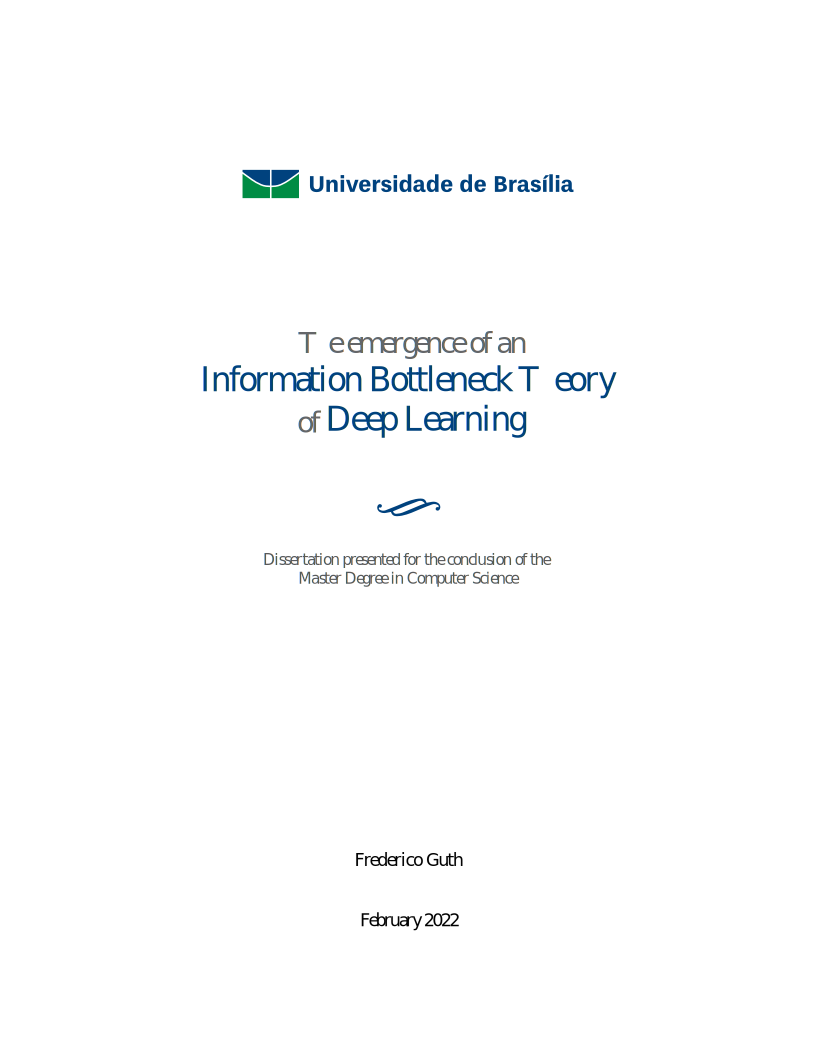
\includepdf{Images/cover.pdf}
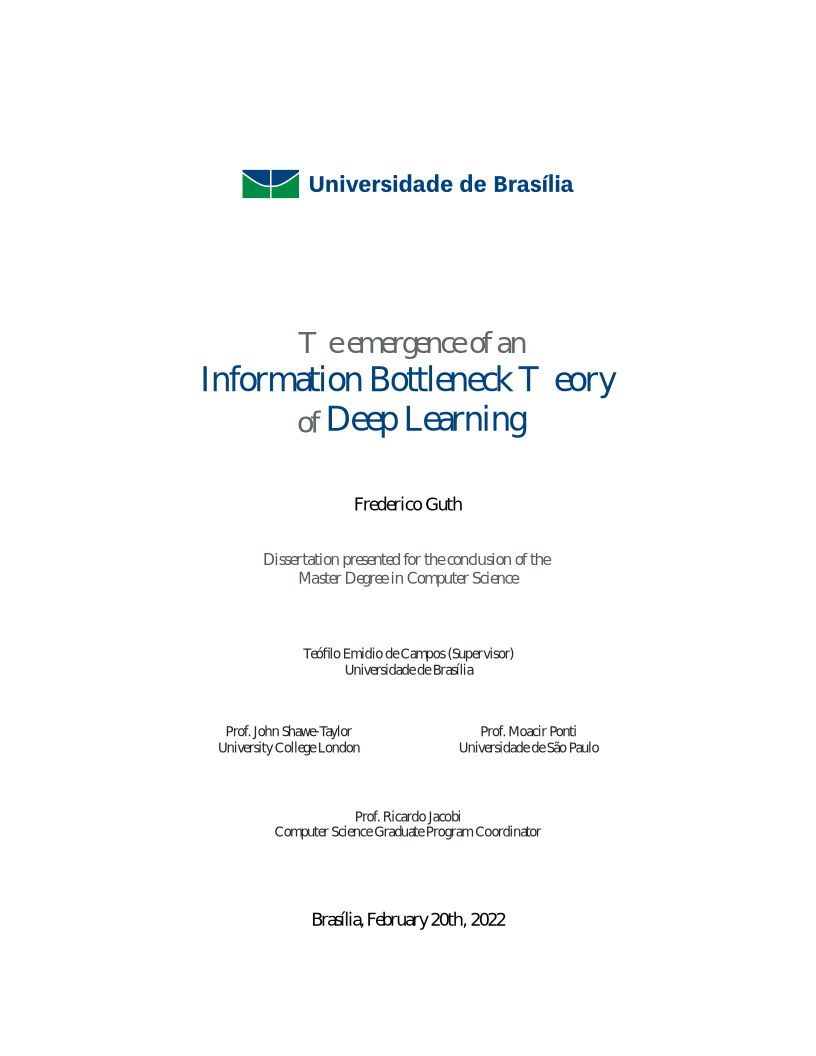
\includepdf{Images/coversheet.pdf} 
%  TODO: remove/change maketitle if cover present
% %%%%%%%%%%%%%%%%%%%%%%%%%%%%%%%%%%%%%%%%%%%%%%%%%%%%%%%%%%%%%%%%%%%%%%%%%%%%%%%%
% r.1 blank page
\clearpage

% v.2 epigraphs
\newpage\thispagestyle{empty}
\openepigraph{%
The public is more familiar with bad design than good design.
It is, in effect, conditioned to prefer bad design, 
because that is what it lives with. 
The new becomes threatening, the old reassuring.
}{Paul Rand%, {\itshape Design, Form, and Chaos}
}
\vfill
\openepigraph{%
A designer knows that he has achieved perfection 
not when there is nothing left to add, 
but when there is nothing left to take away.
}{Antoine de Saint-Exup\'{e}ry}
\vfill
\openepigraph{%
\ldots the designer of a new system must not only be the implementor and the first 
large-scale user; the designer should also write the first user manual\ldots 
If I had not participated fully in all these activities, 
literally hundreds of improvements would never have been made, 
because I would never have thought of them or perceived 
why they were important.
}{Donald E. Knuth}


% v.4 copyright page
\newpage
\begin{fullwidth}
~\vfill
\thispagestyle{empty}
\setlength{\parindent}{0pt}
\setlength{\parskip}{\baselineskip}
Copyright \copyright\ \the\year\ \thanklessauthor

\par\smallcaps{Published by \thanklesspublisher}

\par\smallcaps{tufte-latex.github.io/tufte-latex/}

\par Licensed under the Apache License, Version 2.0 (the ``License''); you may not
use this file except in compliance with the License. You may obtain a copy
of the License at \url{http://www.apache.org/licenses/LICENSE-2.0}. Unless
required by applicable law or agreed to in writing, software distributed
under the License is distributed on an \smallcaps{``AS IS'' BASIS, WITHOUT
WARRANTIES OR CONDITIONS OF ANY KIND}, either express or implied. See the
License for the specific language governing permissions and limitations
under the License.\index{license}

\par\textit{First printing, \monthyear}
\end{fullwidth}


\ifdefined\Shaded\renewenvironment{Shaded}{\begin{tcolorbox}[borderline west={3pt}{0pt}{shadecolor}, boxrule=0pt, frame hidden, interior hidden, sharp corners, breakable, enhanced]}{\end{tcolorbox}}\fi

\renewcommand*\contentsname{Contents}
{
\hypersetup{linkcolor=}
\setcounter{tocdepth}{1}
\tableofcontents
}
\mainmatter
\bookmarksetup{startatroot}

\hypertarget{welcome}{%
\chapter*{Welcome}\label{welcome}}

\markboth{Welcome}{Welcome}

\bookmarksetup{startatroot}

\hypertarget{section}{%
\chapter{}\label{section}}

\begin{fullwidth}
~\vfill
\thispagestyle{empty}
\setlength{\parindent}{0pt}
\setlength{\parskip}{\baselineskip}
Copyright \copyright\ \the\year\ \thanklessauthor

\par\smallcaps{Published by \thanklesspublisher}

\par\smallcaps{tufte-latex.github.io/tufte-latex/}

\par Licensed under the Apache License, Version 2.0 (the ``License''); you may not
use this file except in compliance with the License. You may obtain a copy
of the License at \url{http://www.apache.org/licenses/LICENSE-2.0}. Unless
required by applicable law or agreed to in writing, software distributed
under the License is distributed on an \smallcaps{``AS IS'' BASIS, WITHOUT
WARRANTIES OR CONDITIONS OF ANY KIND}, either express or implied. See the
License for the specific language governing permissions and limitations
under the License.\index{license}

\par\textit{First printing, \monthyear}
\end{fullwidth}

\bookmarksetup{startatroot}

\hypertarget{dedication}{%
\chapter{Dedication}\label{dedication}}

\emph{This work is dedicated to my beloved wife, Júlia.} \vfill

\begin{quote}
O correr da vida embrulha tudo.\\
A vida é assim:\\
esquenta e esfria,\\
aperta e daí afrouxa,\\
sossega e depois desinquieta.\\
O que ela quer da gente é coragem\\
\strut \\
--- Guimarães Rosa
\end{quote}

\bookmarksetup{startatroot}

\hypertarget{acknowledgements}{%
\chapter{Acknowledgements}\label{acknowledgements}}

This dissertation would not have been possible without the help of many
people. I am very thankful to Teo de Campos, my supervisor, for the
support and encouragement even when my interests led the work far from
his comfort zone. I also thank my committee members, John Shawe-Taylor
and Moacir Ponti, for investing the time to read and evaluate a
dissertation that was way longer than expected.

Many thanks to my colleagues, especially Pedro Luz and Aloísio Dourado,
for the collaboration and stimulating discussions. I am in- debted also
to several UnB teachers: Daniel Guerreiro, Thiago Faleiros, Fabrício
Braz, Li Weigang, Bruno Espinoza, Anderson Nascimento and many others.
In particular, I want to thank Célia Ralha for all the kindness and
guidance.

I thank everybody from the Knedle project and the LISA lab. I am also
grateful for the support from Fundação de Apoio à Pesquisa do Distrito
Federal(FAPDF\footnote{Conference on Neural Information Processing.})
and Fundação de Empreendimentos Científicos e Tecnológicos (FINATEC).

I also acknowledge that without the bravery of Alexandra Elbakyan of
Sci-hub, this would be a much poorer dissertation. I also would like to
thank Friedrich Wiemer, Cassiano Rabelo and Aaron Turon. Without relying
on their work2, I would never be able to de- velop the complex aesthetic
of this document.

I need to thank my loved ones. My friends Gabriel Squeff, Eduardo
Dimitrov and Erick Muzart read this dissertation's early drafts even
though it is not in their areas of interest. My brother Felipe, whose
patience and support are crucial in all my endeavours. My parents, Leila
and Klaus, and in-laws, Anna, Romero and Alessandro, for mak- ing the
day-to-day life endurable. Lastly, my wife Júlia and daughter Luísa, for
keeping me sane and happy.

\bookmarksetup{startatroot}

\hypertarget{ch:introduction}{%
\chapter{Introduction}\label{ch:introduction}}

In his acceptance speech for the Test-of-Time award in NeurIPS
2017,\footnote{Conference on Neural Information Processing.} Ali
Rahimi\footnote{Research Scientist, Google.} started a controversy by
frankly declaring (Rahimi 2018, 12'10''). His concerns on the lack of
theoretical understanding of machine learning for critical
decision-making are rightful: \textgreater{} \textbar{} `We are building
systems that govern healthcare and mediate our civic dialogue. We would
influence elections. I would like to live in a society whose systems are
built on top of verifiable, rigorous, thorough knowledge and not on
alchemy.'

The next day, Yann LeCun\footnote{Deep Learning pioneer and 2018 Turing
  award winner.
  \url{https://www.facebook.com/yann.lecun/posts/10154938130592143}}
responded: \textgreater{} \textbar{} `Criticising an entire com- munity
(. . .) for practising ``alchemy'', simply because our current
theoretical tools have not caught up with our practice is dangerous.'

Both researchers, at least, agree upon one thing: the practice of
machine learning has outpaced its theoretical development. That is
certainly a research opportunity.

\hypertarget{sec:greeks}{%
\subsection{A Tale of Babylonians and Greeks}\label{sec:greeks}}

\begin{marginfigure}

{\centering 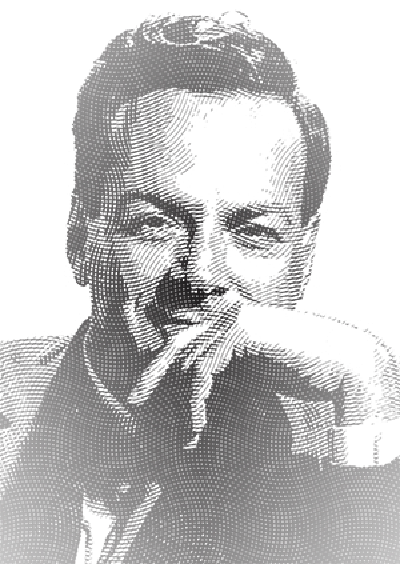
\includegraphics{Chapters/feynman.pdf}

}

\caption{\label{fig-feynman}Richard Feynman, Nobel laureate physicist.}

\end{marginfigure}

Richard Feynman (\protect\hyperlink{fig:feynman}{{[}fig:feynman{]}})
used to lecture this story~(Feynman 1994): Babylonians were pioneers in
mathematics; Yet, the Greeks took the credit. We are used to the Greek
way of doing Math: start from the most basic axioms and build up a
knowledge system. Babylonians were quite the opposite; they were
pragmatic. No knowledge was considered more fundamental than others, and
there was no urge to derive proofs in a particular order. Babylonians
were concerned with the phenomena, Greeks with the ordinance. In
Feynman's view, science is constructed in the Babylonian way. There is
no fundamental truth. Theories try to connect dots from different pieces
of knowledge. Only as science advances, one can worry about
reformulation, simplification and ordering. Scientists are Babylonians;
mathematicians are Greeks.

Mathematics and science are both tools for knowledge acquisition. They
are also social constructs that rely on peer-reviewing. They are
somewhat different, however.

Science is empiric, based on facts collected from \textbf{experience}.
When physicists around the world measured events that corroborated
Newton's \emph{``Law of Universal Gravitation''}, they did not prove it
correct; they just made his theory more and more plausible. Still, only
one experiment was needed to show that Einstein's \emph{Relativity
Theory} was even more believable. In contrast, we can and do prove
things in mathematics.

In mathematics, knowledge is absolute truth, and the way one builds new
knowledge with it, its inference method, is deduction. Mathematics is a
language, a formal one, a tool to precisely communicate some kinds of
thoughts. As it happens with natural languages, there is beauty in it.
The mathematician expands the boundaries of expression in this language.

In science, there are no axioms: a falsifiable hypothesis/theory is
proposed, and logical conclusions (predictions) from the theory are
empirically tested. Despite inferring hypotheses by induction, there is
no influence of psychology in the process. A tested hypothesis is not
absolute truth. A hypothesis is never verified, only falsified by
experiments~(Popper 2004, 31--50). Scientific knowledge is belief
justified by experience; there are degrees of plausibility.

Understanding the epistemic contrast between mathematics and science
will help us understand the past of {AI} and avoid some perils in its
future.

\hypertarget{the-importance-of-theoretical-narratives}{%
\subsection{The importance of theoretical
narratives}\label{the-importance-of-theoretical-narratives}}

\textbf{Science is a narrative} of how we understand Nature~(Gleiser and
Sowinski 2018). In science, we collect facts, but they need
interpretation. The logical conclusion from the hypothesis that predicts
some behaviour in nature gives a plausible \emph{meaning} to what we
observed.

To illustrate, take the ancient human desire of flying. There have
always been stories of men strapping wings to themselves and attempting
to fly by jumping from a tower and flapping those wings like birds (see
Farrington 2016). While concepts like lift, stability, and control were
poorly understood, most human flight attempts ended in severe injury or
even death. It did not matter how much evidence, how many hours of
seeing different animals flying, those ludicrous brave men experienced;
the \emph{meaning} they took from what they saw was wrong, and their
predictions incorrect.

They did not die in vain\footnote{Those ``researchers'' deserved, at
  least, a Darwin Award of Science. The Darwin Award is satirical
  honours that recognise individuals who have unwillingly contributed to
  human evolution by selecting themselves out of the gene pool.};
Science advances when scientists are wrong. Theories must be
falsifiable, and scientists cheer for their failure. When it fails,
there is room for new approaches. Only when we understood the
observations in animal flight from the aerodynamics perspective, we
learned to fly better than any other animal before. Science works by a
``natural selection'' of ideas, where only the fittest ones survive
until a better one is born. Chaitin also points out that an idea has
``fertility'' to the extent to which it ``illuminates us, inspires us
with other ideas, and suggests unsuspected connections and new
viewpoints''~(Chaitin 2006, 9).

Being a Babylonian enterprise, science has no clear path. One of the
exciting facts one can learn by studying its history is that robust
discoveries have arisen through the study of phenomena in human-made
devices~(Pierce, n.d.). For instance, Carnot's first and only scientific
work~(Klein 1974) gave birth to thermodynamics: the study of energy, the
conversion between its different forms, and the ability of energy to do
work;~the science that explains how steam engines work. However, steam
engines came before Carnot's work and were studied by him. Such
human-made devices may present a simplified instance of more complex
natural phenomena.

Another example is Information Theory. Several insights of Shannon's
theory of communication were generalisations of ideas already present in
Telegraphy~(Shannon 1948). New theories in artificial intelligence can,
therefore, be developed from insights in the study of deep learning
phenomena.\footnote{Understanding human intelligence using artificial
  intelligence is a field of study called Computational Neuroscience.}

\hypertarget{sec:bringing_science}{%
\subsection{Bringing science to Computer
Science}\label{sec:bringing_science}}

Despite the name, Computer Science has been more mathematics than
science. We, computer scientists, are very comfortable with theorems and
proofs, not much with theories.

Nevertheless, {AI} has essentially become a Babylonian enterprise, a
scientific endeavour. Thus, there is no surprise when some computer
scientists still see AI with some distrust and even disdain, despite its
undeniable usefulness:

\begin{itemize}
\item
  Even among AI researchers, there is a trend of ``mathiness'' and
  speculation disguised as explanations in conference papers~(Lipton and
  Steinhardt 2018).
\item
  There are few venues for papers that describe surprising phenomena
  without trying to come up with an explanation. As if the mere
  inconsistency of the current theoretical framework was unworthy of
  publication.
\end{itemize}

While physicists rejoice in finding phenomena that contradict current
theories, computer scientists get baffled. In Natural Sciences,
unexplained phenomena lead to theoretical development. Some believe they
bring \emph{winters}, periods of progress stagnation and lack of funding
in {AI}.\footnote{This seems to be Yann LeCun's opinion: However, due to
  all possible alternative explanations (lack of computational power, no
  availability of massive annotated datasets), it seems harsh or simply
  wrong to blame theorists.}

Artificial Intelligence has been through several of the aforementioned
``winters''. In 1957, Herbert Simon\footnote{Herbert Simon
  (\(1916\)--\(2001\)) received the Turing Award in \(1975\), and the
  Nobel Prize in Economics in \(1978\).} famously predicted that within
ten years, a computer would be a chess champion~(Russell, Norvig, and
Davis 2010, sec. 1.3). It took around 40 years, in any case. Computer
scientists lacked understanding of the exponential nature of the
problems they were trying to solve: Computational Complexity Theory had
yet to be invented.

Machine Learning Theory (computational and statistical) tries to avoid a
similar trap by analysing and classifying learning problems according to
the number of samples required to learn them (besides the number of
steps). The matter of concern is that it currently predicts that
generalisation requires simpler models in terms of parameters. In total
disregard to the theory, deep learning models have shown spectacular
generalisation power with hundreds of millions of parameters (and even
more impressive overfitting capacity~).

\hypertarget{problem}{%
\section{Problem}\label{problem}}

In the last decade, we have witnessed a myriad of astonishing successes
in Deep Learning. Despite those many successes in research and industry
applications, we may again be climbing a peak of inflated expectations.
If in the past, the false solution was to ``add computation power'' on
problems, today we try to solve them by ``piling
data''(\protect\hyperlink{fig:machine_learning_2x}{{[}fig:machine\_learning\_2x{]}}).
Such behaviour has triggered a winner-takes-all competition for who
collects more data (our data) amidst a handful of large corporations,
raising ethical concerns about privacy and concentration of
power~(O'Neil 2016).

Nevertheless, we know that learning from way fewer samples is possible:
humans show a much better generalisation ability than our current
state-of-the-art artificial intelligence. To achieve such needed
generalisation power, we may need to understand better how learning
happens in deep learning. Rethinking generalisation might reshape the
foundations of machine learning theory~(Zhang et al. 2016).

\hypertarget{possible-new-explanation-in-the-horizon}{%
\subsection{Possible new explanation in the
horizon}\label{possible-new-explanation-in-the-horizon}}

In \(2015\), ~Tishby and Zaslavsky (2015) proposed a theory of deep
learning ~(Tishby and Zaslavsky 2015) based on the
information-theoretical concept of the bottleneck principle, of which
Tishby is one of the authors. Later, in 2017, ~Shwartz-Ziv and Tishby
(2017) followed up on the {IBT} with the paper ~, which was presented in
a well-attended workshop\footnote{Deep Learning: Theory, Algorithms, and
  Applications. Berlin, June 2017
  \url{http://doc.ml.tu-berlin.de/dlworkshop2017}}, with appealing
visuals that clearly showed a \emph{``phase transition''} happening
during training. The video posted on Youtube~(Tishby 2017) became a
``sensation''\footnote{By the time of this writing, this video as more
  than \(84,000\) views, which is remarkable for an hour-long workshop
  presentation in an academic niche. \url{https://youtu.be/bLqJHjXihK8}},
and received a wealth of publicity when well-known researchers like
Geoffrey Hinton\footnote{Another Deep Learning Pioneer \textbf{and}
  Turing award winner (2018).}, Samy Bengio (Apple) and Alex Alemi
(Google Research) have expressed interest in Tishby's ideas~(Wolchover
2017). they are called formal languages.

\begin{quote}
\emph{I believe that the information bottleneck idea could be very
important in future deep neural network research.} --- Alex Alemi
\end{quote}

Andrew Saxe (Harvard University) rebutted ~Shwartz-Ziv and Tishby (2017)
claims in ~ and was followed by other critics. According to Saxe, it was
impossible to reproduce ~(Shwartz-Ziv and Tishby 2017)'s experiments
with different parameters.

\emph{Has the initial enthusiasm on the {IBT} been unfounded? Have we
let us ``fool ourselves'' by beautiful charts and a good story?}

\hypertarget{problem-statement}{%
\subsection{Problem statement}\label{problem-statement}}

\textbf{The practice of modern machine learning has outpaced its
theoretical development.} In particular, deep learning models present
generalisation capabilities unpredicted by the current machine learning
theory. There is yet no established new general theory of learning which
handles this problem.

{IBT} was proposed as a possible new theory with the \textbf{potential}
of filling the theory-practice gap. Unfortunately, to the extent of our
knowledge, \textbf{there is still no comprehensive digest of {IBT} nor
an analysis of how it relates to current {MLT}}.

\hypertarget{objective}{%
\section{Objective}\label{objective}}

This dissertation aims to investigate \emph{to what extent} can the
emergent Information Bottleneck Theory help us better understand Deep
Learning and its phenomena, especially generalisation, presenting its
strengths, weaknesses and research opportunities.

\hypertarget{research-questions}{%
\subsection{Research Questions}\label{research-questions}}

\hypertarget{methodology}{%
\section{Methodology}\label{methodology}}

\begin{enumerate}
\def\labelenumi{\arabic{enumi}.}
\item
  Given that {IBT} is yet not a well-established learning theory, there
  were two difficulties that the research had to address:

  \begin{enumerate}
  \def\labelenumii{\arabic{enumii}.}
  \item
    There is a growing interest in the subject, and new papers are
    published every day. It was essential to select literature and
    restrain the analysis.
  \item
    Early on, the marks of an emergent theory in its infancy manifested
    in the form of missing assumptions, inconsistent notation, borrowed
    jargon, and seeming missing steps. Foremost, it was unclear what was
    missing from the theory and what was missing in our understanding.
  \end{enumerate}

  An initial literature review on {IBT} was conducted to define the
  scope.\footnote{Not even the term {IBT} is universally adopted.} We
  then chose to narrow the research to \textbf{theoretical perspective
  on generalisation}, where we considered that it could bring
  fundamental advances. We made the deliberate choice of going deeper in
  a limited area of {IBT} and not broad, leaving out a deeper
  experimental and application analysis, all the work on
  {ITL}\footnote{{ITL} makes the opposite path we are taking, bringing
    concepts of machine learning to information theory problems.}
  ~(Principe 2010) and statistical-mechanics-based analysis of SGD ~(P.
  Chaudhari and Soatto 2018; Pratik Chaudhari et al. 2019). From this
  set of constraints, we chose a list of pieces of {IBT} literature to
  go deeper (\protect\hyperlink{ch:literature}{{[}ch:literature{]}}).
\item
  In order to answer , we discuss the epistemology of {AI} to choose
  fundamental axioms (definition of intelligence and the definition of
  knowledge) with which we deduced from the ground up {MLT}, {IT} and
  {IBT}, revealing hidden assumptions, pointing out similarities and
  differences. By doing that, we built a ``genealogy'' of these research
  fields. This comparative study was essential for identifying missing
  gaps and research opportunities.
\item
  In order to answer , we first dissected the selected literature
  (\protect\hyperlink{ch:literature}{{[}ch:literature{]}}) and organised
  scattered topics in a comprehensive sequence of subjects.
\item
  In the process of the literature digest, we identified results,
  strengths, weaknesses and research opportunities.
\end{enumerate}

\hypertarget{contributions}{%
\section{Contributions}\label{contributions}}

In the research conducted, we produced three main results that, to the
extent of our knowledge, are original:

\begin{enumerate}
\def\labelenumi{\arabic{enumi}.}
\item
  The dissertation itself is the main expected result: a comprehensive
  digest of the {IBT} literature and a snapshot analysis of the field in
  its current form, focusing on its theoretical implications for
  generalisation.
\item
  We propose an Information-Theoretical learning problem different from
  {MDL} proposed by ~(Hinton and Van Camp 1993) for which we derived
  bounds using Shannon's . These results, however, are only indicative
  as they lack peer review to be validated.
\item
  We present a critique on Achille (2019)'s explanation~(Achille 2019;
  Achille and Soatto 2018) for the role of layers in Deep Representation
  in the {IBT}
  perspective~(\protect\hyperlink{sec:achille_proof_critique}{{[}sec:achille\_proof\_critique{]}}),
  pointing out a weakness in the argument that, as far as we know, has
  not yet been presented. We then propose a counter-intuitive
  \emph{hypothesis} that layers reduce the model's ``effective''
  hypothesis space. This \emph{hypothesis} is not formally proven in the
  present work, but we try to give the intuition behind it
  (\protect\hyperlink{sec:proposed_hypothesis}{{[}sec:proposed\_hypothesis{]}}).
  This result has not yet been validated as well.
\end{enumerate}

\hypertarget{dissertation-preview-and-outline}{%
\section{Dissertation preview and
outline}\label{dissertation-preview-and-outline}}

The dissertation is divided into two main parts
(\protect\hyperlink{pt:background}{{[}pt:background{]}} and
\protect\hyperlink{pt:emergence_of_theory}{{[}pt:emergence\_of\_theory{]}}),
with a break in the middle
(\protect\hyperlink{pt:intermezzo}{{[}pt:intermezzo{]}}).

\begin{enumerate}
\def\labelenumi{\arabic{enumi}.}
\item
  Background (\protect\hyperlink{pt:background}{{[}pt:background{]}})

  \begin{itemize}
  \item
    Chapter 2--Artificial Intelligence: The chapter defines what
    artificial intelligence is, presents the epistemological differences
    of intelligent agents in history, and discusses their consequences
    to machine learning theory.
  \item
    Chapter 3 --- Probability Theory: The chapter derives propositional
    calculus and probability theory from a list of desired
    characteristics for epistemic agents. It also presents basic
    Probability Theory concepts.
  \item
    Chapter 4 --- Machine Learning Theory: The chapter presents the
    theoretical framework of Machine Learning, the PAC model,
    theoretical guarantees for generalisation, and expose its weaknesses
    concerning Deep Learning phenomena.
  \item
    Chapter 5 --- Information Theory: The chapter derives Shannon
    Information from Probability Theory, explicates some implicit
    assumptions, and explains basic Information Theory concepts.
  \end{itemize}
\item
  Intermezzo (\protect\hyperlink{pt:intermezzo}{{[}pt:intermezzo{]}})

  \begin{itemize}
  \tightlist
  \item
    Chapter 6 --- Information-Theoretical Epistemology: This chapter
    closes the background part and opens the IBT part of the
    dissertation. It shows the connection of {IT} and {MLT} in the
    learning problem, proves that Shannon theorems can be used to prove
    PAC bounds and present the {MDL} Principle, an earlier example of
    this kind of connection.
  \end{itemize}
\item
  The emergence of a theory
  (\protect\hyperlink{pt:emergence_of_theory}{{[}pt:emergence\_of\_theory{]}})

  \begin{itemize}
  \item
    Chapter 7 --- IB Principle: Explains the IB method and its tools:
    {KL} as a natural distortion (loss) measure, the IB Lagrangian and
    the Information Plane.
  \item
    Chapter 8 --- IB and Representation Learning: Presents the learning
    problem in the {IBT} perspective (not specific to {DL}). It shows
    how some usual choices of the practice of {DL} emerge naturally from
    a list of desired properties of representations. It also shows that
    the information in the weights bounds the information in the
    activations.
  \item
    Chapter 9 --- IB and Deep Learning: This chapter presents the {IBT}
    perspective specific to Deep Learning. It presents {IBT} analysis of
    Deep Learning training, some examples of applications of {IBT} to
    improve or create algorithms; and the {IBT} learning theory of Deep
    Learning. We also explain Deep Learning phenomena in the {IBT}
    perspective.
  \item
    Chapter 10 --- Conclusion: In this chapter, we present a summary of
    the findings, answer the research questions, and present suggestions
    for future work.
  \end{itemize}
\end{enumerate}

We found out that {IBT} does not invalidate {MLT}; it just interprets
complexity not as a function of the data (number of parameters) but as a
function of the information contained in the data. With this
interpretation, there is no paradox in improving generalisation by
adding layers.

Furthermore, they both share more or less the same ``genealogy'' of
assumptions. {IBT} can be seen as particular case of {MLT}.
Nevertheless, {IBT} allows us to better understand the training process
and provide a different narrative that helps us comprehend Deep Learning
phenomena in a more general way.

\hypertarget{refs}{}
\begin{CSLReferences}{1}{0}
\leavevmode\vadjust pre{\hypertarget{ref-achille:2019phd}{}}%
Achille, Alessandro. 2019. {``Emergent Properties of Deep Neural
Networks.''} PhD thesis, UCLA.
\url{https://escholarship.org/uc/item/8gb8x6w9}.

\leavevmode\vadjust pre{\hypertarget{ref-achille:2017emergence}{}}%
Achille, Alessandro, and Stefano Soatto. 2018. {``Emergence of
Invariance and Disentangling in Deep Representations.''} \emph{J. Mach.
Learn. Res.} 19 (1): 1947--80.

\leavevmode\vadjust pre{\hypertarget{ref-chaitin:2006}{}}%
Chaitin, Gregory. 2006. \emph{Meta Math! The Quest for Omega}. Vintage
Books.

\leavevmode\vadjust pre{\hypertarget{ref-chaudhari:2019}{}}%
Chaudhari, Pratik, Anna Choromanska, Stefano Soatto, Yann LeCun, Carlo
Baldassi, Christian Borgs, Jennifer Chayes, Levent Sagun, and Riccardo
Zecchina. 2019. {``Entropy-Sgd: Biasing Gradient Descent into Wide
Valleys.''} \emph{Journal of Statistical Mechanics: Theory and
Experiment} 2019 (12).

\leavevmode\vadjust pre{\hypertarget{ref-chaudhari:2018SGD}{}}%
Chaudhari, P., and S. Soatto. 2018. {``Stochastic Gradient Descent
Performs Variational Inference, Converges to Limit Cycles for Deep
Networks.''} In \emph{2018 Information Theory and Applications Workshop
(ITA)}, 1--10. \url{https://doi.org/10.1109/ITA.2018.8503224}.

\leavevmode\vadjust pre{\hypertarget{ref-farrington:2016}{}}%
Farrington, Karen. 2016. \emph{The Blitzed City: The Destruction of
Coventry, 1940}. London: Aurum Press.

\leavevmode\vadjust pre{\hypertarget{ref-feynman:1994}{}}%
Feynman, Richard. 1994. \emph{The Character of Physical Law}. Modern
Library.

\leavevmode\vadjust pre{\hypertarget{ref-gleiser:2018}{}}%
Gleiser, Marcelo, and Damian Sowinski. 2018. {``The Map and the
Territory.''} In \emph{The Frontiers Collection}, edited by Shyam
Wuppuluri and Francisco Antonio Doria. Springer International
Publishing. \url{https://doi.org/10.1007/978-3-319-72478-2}.

\leavevmode\vadjust pre{\hypertarget{ref-hinton:1993}{}}%
Hinton, Geoffrey E, and Drew Van Camp. 1993. {``Keeping the Neural
Networks Simple by Minimizing the Description Length of the Weights.''}
In \emph{Proceedings of the Sixth Annual Conference on Computational
Learning Theory}, 5--13.

\leavevmode\vadjust pre{\hypertarget{ref-klein:1974}{}}%
Klein, Martin J. 1974. {``Carnot{\textquotesingle}s Contribution to
Thermodynamics.''} \emph{Physics Today} 27 (8): 23--28.
\url{https://doi.org/10.1063/1.3128802}.

\leavevmode\vadjust pre{\hypertarget{ref-lipton:2018}{}}%
Lipton, Zachary C., and Jacob Steinhardt. 2018. {``Troubling Trends in
Machine Learning Scholarship.''} \url{https://arxiv.org/abs/1807.03341}.

\leavevmode\vadjust pre{\hypertarget{ref-oneil:2016}{}}%
O'Neil, Cathy. 2016. \emph{Weapons of Math Destruction: How Big Data
Increases Inequality and Threatens Democracy}. USA: Crown Publishing
Group.

\leavevmode\vadjust pre{\hypertarget{ref-pierce:1980}{}}%
Pierce, John R. n.d. \emph{An Introduction to Information Theory:
Symbols, Signals and Noise}. Dover Publications.

\leavevmode\vadjust pre{\hypertarget{ref-popper:2004}{}}%
Popper, Karl. 2004. \emph{A Lógica Da Pesquisa Científica}. Translated
by Leonidas Hegenberg and Octanny Silveira. São Paulo: Cultrix.

\leavevmode\vadjust pre{\hypertarget{ref-principe:2010}{}}%
Principe, Jose C. 2010. \emph{Information Theoretic Learning: Renyi's
Entropy and Kernel Perspectives}. Springer Science \& Business Media.

\leavevmode\vadjust pre{\hypertarget{ref-rahimi:2017}{}}%
Rahimi, Ali. 2018. {``Ali Rahimi NIPS 2017 Test-of-Time Award
Presentation Speech.''} \url{https://youtu.be/x7psGHgatGM}; Youtube.
\url{https://youtu.be/x7psGHgatGM}.

\leavevmode\vadjust pre{\hypertarget{ref-russell:2010}{}}%
Russell, Stuart J., Peter Norvig, and Ernest Davis. 2010.
\emph{Artificial Intelligence: A Modern Approach}. 3rd ed. Prentice
{{Hall} } Series in Artificial Intelligence. Prentice Hall.

\leavevmode\vadjust pre{\hypertarget{ref-shannon:1948}{}}%
Shannon, Claude E. 1948. {``A Mathematical Theory of Communication.''}
\emph{Bell System Technical Journal} 27 (3): 379--423.

\leavevmode\vadjust pre{\hypertarget{ref-shwartz-ziv:2017}{}}%
Shwartz-Ziv, Ravid, and Naftali Tishby. 2017. {``Opening the Black Box
of Deep Neural Networks via Information.''}
\url{https://arxiv.org/abs/1703.00810}.

\leavevmode\vadjust pre{\hypertarget{ref-tishby:2017yt1}{}}%
Tishby, Naftali. 2017. {``Information Theory of Deep Learning.''}
\url{https://youtu.be/bLqJHjXihK8}. \url{https://youtu.be/bLqJHjXihK8}.

\leavevmode\vadjust pre{\hypertarget{ref-tishby:2015dlib}{}}%
Tishby, Naftali, and Noga Zaslavsky. 2015. {``Deep Learning and the
Information Bottleneck Principle.''} In \emph{2015 IEEE Information
Theory Workshop (ITW)}, 1--5. IEEE.

\leavevmode\vadjust pre{\hypertarget{ref-wolchover:2017quanta}{}}%
Wolchover, Natalie. 2017. {``New Theory Cracks Open the Black Box of
Deep Learning.''}
\url{https://www.quantamagazine.org}/new-theory-cracks-open-the-black-box-of-deep-learning-20170921/;
Simons Foundation.

\leavevmode\vadjust pre{\hypertarget{ref-zhang:2016}{}}%
Zhang, Chiyuan, Samy Bengio, Moritz Hardt, Benjamin Recht, and Oriol
Vinyals. 2016. {``Understanding Deep Learning Requires Rethinking
Generalization.''} \url{https://arxiv.org/abs/1611.03530}.

\end{CSLReferences}


\backmatter

\end{document}
